\documentclass{article}
\usepackage[left=2cm,right=2cm,top=3cm,bottom=3cm,letterpaper]{geometry}
\usepackage[spanish]{babel}
\usepackage[utf8]{inputenc}
\usepackage{graphicx}
\usepackage{enumitem}
\usepackage{hyperref}

\title{Prueba y Comparación de Naive Bayes y C4.5}
\author{Juan Carlos López López \and Adolfo Marín Arriaga \and Luis Rodrigo Rojo Morales}
\date{\today\\}
\begin{document}
 \maketitle
 \section{Introducción}
 Para hacer las pruebas de estos algoritmos usamos el conjunto de datos que esta destinado a probar los clasificadores, este se puede obtener en: \href{https://archive.ics.uci.edu/ml/datasets/Adult} {https://archive.ics.uci.edu/ml/datasets/Adult} y en nuestro repositorio se encuentra en: \href{https://github.com/rodrigorojo/ProyectoFinalMineria/blob/master/Entregable3/NaiveBayes/AdultDataSetTest.csv}{/Entregable3/NaiveBayes/AdultDataSetTest.csv}. Dicho conjunto tiene 16,281 registros, los cuales cada uno tiene los mismos atributos que el conjunto de datos original.

 \section{Naive Bayes}
 El script para probar este clasificador se encuentra en \href{https://github.com/rodrigorojo/ProyectoFinalMineria/blob/master/Entregable3/NaiveBayes/TestAdultDataSet.java} {/Entregable3/NaiveBayes/TestAdultDataSet.java} el objetivo de este script es cargar el conjunto de datos prueba, aplicar el clasificador y dar los datos de cuantos clasifico bien y cuantos mal, para así poder hacer la matriz de confusión, la cual queda de la siguiente manera:
 \begin{center}
   \begin{tabular}{|p{2cm}|p{2cm}|p{2cm}|}
     \hline
                  & $>$ 50K & $\leq$ 50K  \\ \hline
      $>$ 50K     & 3023 & 823 \\ \hline
      $\leq$ 50K  & 2201 & 10234 \\ \hline
    \end{tabular}
 \end{center}
 Con esta matriz podemos observar que el clasificador predijo 13257 bien y 3024 mal, a 823 personas le dijimos que iban a ganar $\leq$ 50K pero en realidad ganaron $>$ 50K, mientras que a 2201 personas les dijimos que iban a ganar $>$ 50K pero ganaron $\leq$ 50K.

 El clasificador en general tiene una exactitud del 81.7$\%$, mientras que individualmente predice a los que ganan más de 50K con una exactitud de 57.86$\%$ y a los que ganan menos o 50K con una exactitud de 74.43$\%$
 \section{C4.5}

 El script para probar este clasificador se encuentra en \href{https://github.com/rodrigorojo/ProyectoFinalMineria/blob/master/Entregable3/NaiveBayes/TestAdultDataSet.java} {/Entregable3/C4.5/TestAdultDataSet.java} el objetivo de este script es cargar el conjunto de datos prueba, aplicar el clasificador y dar los datos de cuantos clasifico bien y cuantos mal, para así poder hacer la matriz de confusión, la cual queda de la siguiente manera:
 \begin{center}
   \begin{tabular}{|p{2cm}|p{2cm}|p{2cm}|}
     \hline
                  & $>$ 50K & $\leq$ 50K  \\ \hline
      $>$ 50K     & 2168    & 1648         \\ \hline
      $\leq$ 50K  & 689    & 11746        \\ \hline
    \end{tabular}
 \end{center}
 Con esta matriz podemos observar que el clasificador predijo 13914 bien y 2337 mal, a 1648 personas le dijimos que iban a ganar $\leq$ 50K pero en realidad ganaron $>$ 50K, mientras que a 689 personas les dijimos que iban a ganar $>$ 50K pero ganaron $\leq$ 50K.

 El clasificador en general tiene una exactitud del 85.46$\%$, mientras que individualmente predice a los que ganan más de 50K con una exactitud de 56.81$\%$ y a los que ganan menos o 50K con una exactitud de 94.45$\%$
 \section{Comparación}
 Comparando ambas técnicas de clasificación podemos concluir que nive bayes predice mejor a los $>$ 50K mientras que c4.5 predice mejor a $\leq$ 50K, pero en general la técnica de clasificación árboles C4.5 tiene un poco de más precisión.
\begin{center}
  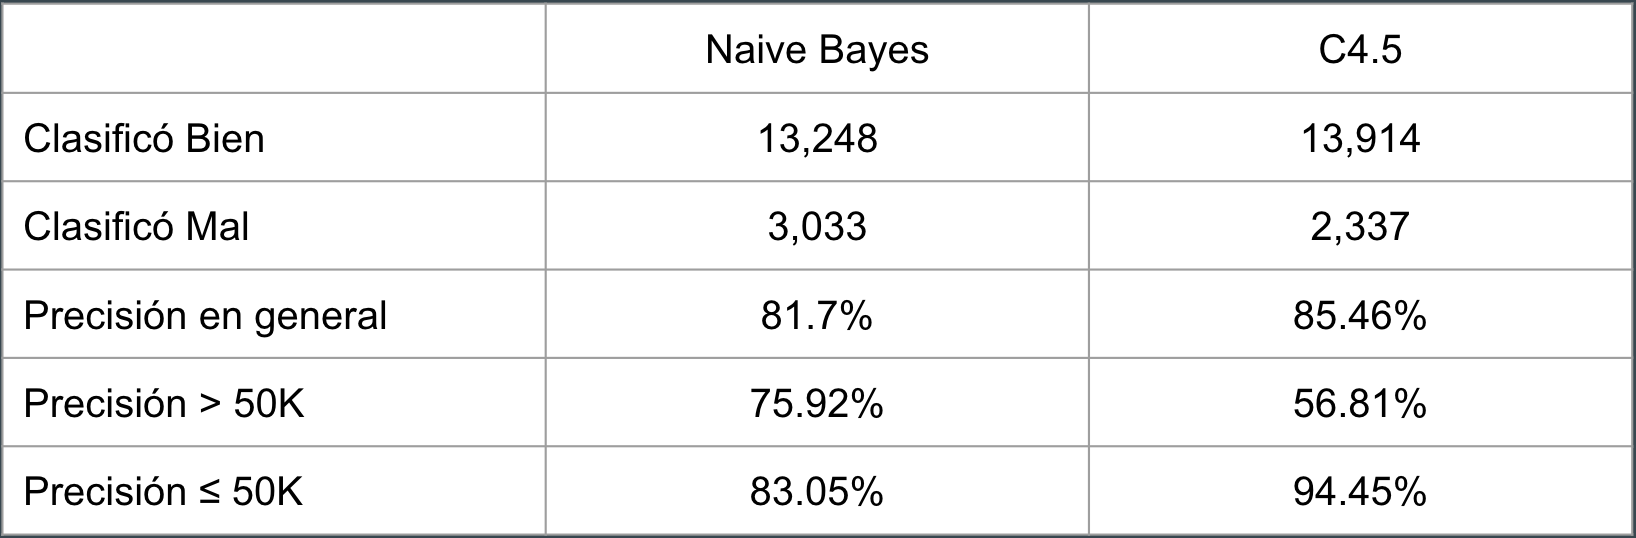
\includegraphics[scale=0.5]{tabla}
\end{center}

\end{document}
